\chapter{Marco Teórico - Conceptual} \label{cap:marco_teorico}

\section{El modelo de red de Kubernetes}

Kubernetes (K8S) no implementa por sí mismo la conectividad entre cargas de trabajo; define un modelo de red y delega su realización en componentes externos. Comprender este modelo es necesario para interpretar las métricas del experimento, dado que el plano de red ---y en particular el plugin que lo implementa--- determina el rendimiento, la seguridad y la eficiencia en la utilización de recursos dentro del clúster~\cite{ref2}.

El modelo de red de Kubernetes establece tres principios fundamentales:
\begin{enumerate}
    \item Cada Pod recibe una dirección de Protocolo de Internet (IP, Internet Protocol) propia y única.
    \item Los Pods se comunican entre sí sin traducción de direcciones de red (NAT, Network Address Translation).
    \item Los agentes del host (como kubelet) alcanzan a todos los Pods ubicados en ese nodo.
\end{enumerate}
Sobre estas garantías se construyen las abstracciones de descubrimiento, balanceo y control de acceso del clúster~\cite{ref2}.

La siguiente analogía ayuda a visualizar cómo interactúan estos componentes:
\begin{itemize}
    \item \textbf{Pods (Viviendas):} Constituyen las residencias particulares del clúster. Cada Pod cuenta con una dirección IP única y efímera que le permite comunicarse directamente con cualquier otra vivienda del entorno sin intermediarios.
    \item \textbf{Nodos (Barrios):} Alojan múltiples viviendas y proveen los recursos físicos y de cómputo (CPU, memoria y conectividad) indispensables para la subsistencia de los servicios.
    \item \textbf{Servicios (Central telefónica):} Operan como un conmutador estable con un número de contacto único e invariable. Esto permite canalizar el tráfico hacia las réplicas adecuadas, independientemente de los cambios internos en su ciclo de vida.
    \item \textbf{Ingress y Gateway API (Portería):} Representan el acceso administrado y seguro desde el exterior (Internet), asegurando el gobierno del tráfico entrante y la separación de responsabilidades funcionales.
\end{itemize}

El sustrato vial que hace posible la comunicación física entre las viviendas y barrios corresponde a la Interfaz de Red de Contenedores (CNI, Container Network Interface), la cual se detalla en la Figura~\ref{fig:red_cluster_k8s} y define la infraestructura de red subyacente.

\begin{figure}[htbp]
    \centering
    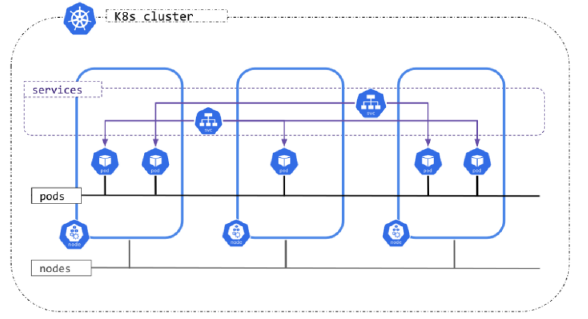
\includegraphics[width=0.85\textwidth]{figures/red_cluster_k8s.png}
    \caption{Topología de red de un clúster de Kubernetes (adaptado de~\cite{ref2}).}
    \label{fig:red_cluster_k8s}
\end{figure}

\subsection{Identidad de red del Pod}

Kubernetes adopta el modelo de direccionamiento IP por Pod, asignando una dirección única a cada unidad de ejecución. Este enfoque facilita que las cargas de trabajo interactúen de forma directa y nativa sin recurrir a NAT. Dado que la identidad del Pod es efímera ---las réplicas se crean, destruyen y sustituyen de manera dinámica por los controladores---, la plataforma requiere abstracciones estables para asegurar el descubrimiento y direccionamiento consistente de los destinos~\cite{ref2}.

\subsection{Nodos y reenvío de paquetes}

Cada nodo (Host o máquina virtual/física) hospeda múltiples Pods y aporta recursos de CPU, memoria y conectividad. En este nivel se instalan las rutas del sistema operativo y los mecanismos de reenvío local que garantizan la entrega de paquetes al Pod de destino, conforme al modelo de red del clúster: alcance directo entre Pods, ausencia de superposición de rangos de red y conectividad bidireccional este-oeste~\cite{ref2}. El agente del plugin de red se ejecuta precisamente en este nivel; por ello, su consumo de CPU y memoria por nodo Worker constituye una de las métricas centrales de la comparativa.

\subsection{Direccionamiento estable: Services y EndpointSlices}

Un Service expone un identificador estable ---una dirección IP virtual (VIP, Virtual IP) conocida como ClusterIP--- que representa a un conjunto de Pods equivalentes. El cliente se conecta a esa IP virtual y la plataforma balancea la solicitud hacia una de las réplicas disponibles, desacoplando a los consumidores de los cambios en el ciclo de vida de los Pods~\cite{ref3,ref13}. 

Para mantener actualizada la relación de destinos, Kubernetes emplea \emph{EndpointSlices}, los cuales mantienen un inventario actualizado de las direcciones IP y puertos de los Pods que respaldan cada Service. Este mecanismo reduce significativamente la sobrecarga de control frente a los antiguos Endpoint monolíticos en clústeres de gran escala~\cite{ref1}. Esta capa es relevante para interpretar la latencia medida: el tiempo en que una solicitud alcanza el Pod correcto comprende tanto la resolución del balanceador (iptables, IPVS o eBPF) como el reenvío realizado por el plugin de red.

\subsection{Ingreso de tráfico externo: Ingress y Gateway API}

El tráfico procedente de Internet no accede directamente a los Pods, sino a través de una capa de ingreso administrada. La \emph{Gateway API} formaliza los roles asociados ---infraestructura, operaciones y desarrollo--- y las reglas de capa 7 (como hostnames, rutas y terminación TLS) que determinan el enrutamiento de cada solicitud hacia el Service correspondiente~\cite{ref17}. 

En despliegues de alta disponibilidad, esta capa suele estar precedida por un balanceador de carga externo de capa 3/4 que distribuye el tráfico antes de que alcance los nodos del clúster~\cite{ref5}.

\subsection{Aislamiento lógico: Namespaces y NetworkPolicies}

Un \emph{Namespace} representa una delimitación lógica dentro del plano de control, orientada a organizar y estructurar recursos por proyectos, equipos o entornos (como desarrollo, pruebas y producción)~\cite{ref2}. Esta separación garantiza la unicidad de nombres DNS internos en la forma \texttt{<servicio>.<namespace>.svc.cluster.local}, lo cual previene ambigüedades en la resolución de nombres~\cite{ref13,ref2}.

Sin embargo, los Namespaces no restringen la comunicación física de red por defecto. La conectividad este-oeste permanece abierta a menos que se definan reglas explícitas de control de acceso mediante NetworkPolicies, aplicando principios de Confianza Cero (\emph{Zero Trust}) para limitar el tráfico exclusivamente a lo autorizado~\cite{ref4,ref24,ref25,ref26}.

Las NetworkPolicies funcionan como firewalls lógicos distribuidos de capa 3/4 que permiten o restringen conexiones basándose en selectores de etiquetas (\emph{labels}), puertos y protocolos, como se ilustra en la Figura~\ref{fig:network_policy}.

\begin{figure}[htbp]
    \centering
    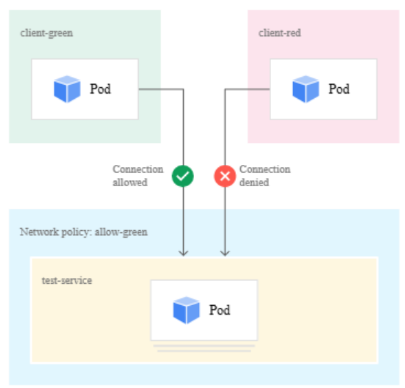
\includegraphics[width=0.85\textwidth]{figures/network_policy.png}
    \caption{Representación de política de red en Kubernetes (NetworkPolicy) con control de conexiones permitidas y denegadas. Fuente: elaboración propia.}
    \label{fig:network_policy}
\end{figure}

Su aplicación efectiva depende de que el CNI implemente el plano de control y de datos correspondiente. Si el plugin CNI seleccionado carece de soporte para NetworkPolicies, la API de Kubernetes aceptará el recurso, pero no se aplicará ninguna regla de seguridad en los nodos, dejando el clúster expuesto~\cite{ref4,ref18}.

\subsection{Recorrido de una solicitud}

El ciclo completo del tráfico responde a la siguiente secuencia operativa:
\begin{enumerate}
    \item El cliente externo envía una solicitud que llega al balanceador y se dirige a la portería lógica (Ingress o Gateway API)~\cite{ref17}.
    \item La portería inspecciona el paquete en capa 7 y lo reenvía al Service adecuado~\cite{ref3,ref13}.
    \item El Service distribuye la petición consultando los EndpointSlices activos para elegir un Pod de destino~\cite{ref1}.
    \item El plugin de red encamina el tráfico hasta el Pod de destino en su nodo correspondiente~\cite{ref2,ref4,ref18}.
\end{enumerate}

\section{La Interfaz de Red de Contenedores (CNI)}

\subsection{Especificación y funciones núcleo}

La especificación Container Network Interface (CNI) define el estándar mediante el cual el runtime de contenedores interactúa con diversos plugins para automatizar la configuración de red. La especificación se fundamenta en operaciones simples y encadenables como la adición (\texttt{ADD}) y la eliminación (\texttt{DEL}) de interfaces de red de los contenedores~\cite{ref18,ref20,ref21,ref28}, un proceso ilustrado esquemáticamente en la Figura~\ref{fig:workflow_cni}.

\begin{figure}[htbp]
    \centering
    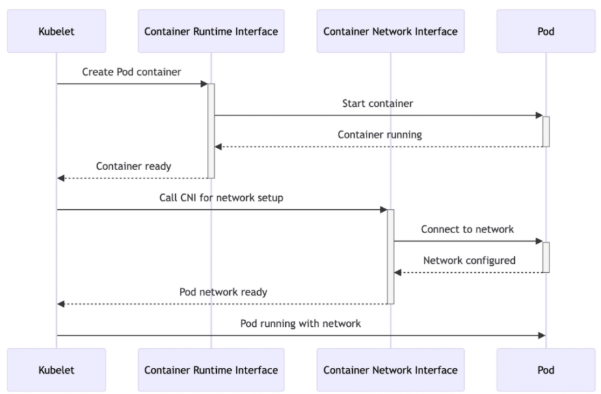
\includegraphics[width=0.85\textwidth]{figures/workflow_cni.png}
    \caption{Diagrama de operación del CNI: interacciones entre Kubelet, Pod y plugins de red.}
    \label{fig:workflow_cni}
\end{figure}

Las funciones básicas que implementa cualquier plugin CNI son:
\begin{itemize}
    \item \textbf{Identidad de Red:} Asignación de IPs del clúster que viabilizan el modelo IP-por-Pod y aseguran la comunicación este-oeste~\cite{ref2}.
    \item \textbf{Enlace e Interfaces:} Creación de veth-pairs para conectar el espacio de nombres de red (\emph{network namespace}) del Pod con la pila de red del host~\cite{ref4,ref18}.
    \item \textbf{Gestión de Direcciones (IPAM):} Reserva y liberación sistemática de direcciones de red a través de componentes como host-local~\cite{ref18,ref20}.
\end{itemize}

\subsection{Modelos de dataplane: redes superpuestas (Overlay) vs. enrutamiento nativo}

El plano de datos del CNI se suele clasificar en dos estrategias principales:
\begin{itemize}
    \item \textbf{Redes Superpuestas (Overlay):} Encapsulan los paquetes de los Pods dentro de protocolos de transporte como VXLAN o Geneve sobre UDP. Esto permite aislar el direccionamiento del clúster de la infraestructura física. Su principal ventaja radica en la simplicidad operativa y el desacoplamiento; a cambio, introduce cabeceras adicionales, posibles ajustes de MTU y cierta carga de CPU por encapsulación/descapsulación.
    \item \textbf{Enrutamiento Nativo (Directo):} Prescinde de túneles lógicos y expone las IPs de los Pods directamente a la red física mediante enrutamiento L3 convencional. Aunque mejora el rendimiento de red y reduce el consumo de CPU, demanda un diseño de direccionamiento rígido y una estrecha integración con la red corporativa.
\end{itemize}

Estudios previos muestran diferencias significativas en el desempeño según el dataplane adoptado, condicionando la viabilidad técnica en entornos con recursos limitados como edge computing o nubes públicas~\cite{ref7,ref8}. En contraste, la aceleración mediante planos de datos avanzados como Open vSwitch (OVS) o programas eBPF (extended Berkeley Packet Filter) incide sustancialmente en la latencia de procesamiento~\cite{ref11,ref22}.

\subsection{Gestión de direcciones (IPAM)}

La gestión de direcciones (IPAM) asigna y libera las IPs de los Pods de forma sistemática; una administración eficiente evita colisiones de red, habilita despliegues dual-stack y sostiene la escalabilidad ante la creación o destrucción masiva de réplicas~\cite{ref18,ref20}.

\subsection{MTU y fragmentación en redes con encapsulación}

En redes superpuestas, el overhead de la encapsulación disminuye el tamaño máximo de segmento de datos útil. Se debe ajustar la Unidad Máxima de Transmisión (MTU, Maximum Transmission Unit) efectiva restando el tamaño de las cabeceras adicionales para prevenir la fragmentación de paquetes, caídas de rendimiento y pérdidas de conexión bajo carga~\cite{ref12}, un proceso ilustrado en la Figura~\ref{fig:ajuste_mtu}.

\begin{figure}[htbp]
    \centering
    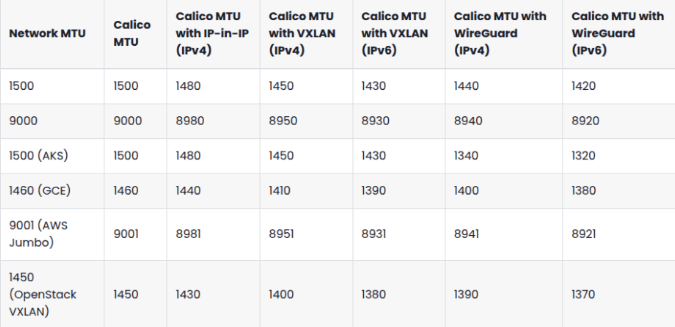
\includegraphics[width=0.85\textwidth]{figures/ajuste_mtu.png}
    \caption{Ajuste de MTU en presencia de encapsulación (p. ej., VXLAN) para evitar fragmentación y pérdida de rendimiento~\cite{ref12}.}
    \label{fig:ajuste_mtu}
\end{figure}

\subsection{Observabilidad del plano de datos}

La operación confiable de microservicios exige visibilidad sobre los flujos de red. Cuando el CNI integra monitoreo de flujos, la telemetría de origen y destino se correlaciona con las identidades nativas del clúster (Namespaces y etiquetas); así, la observabilidad de red se convierte en un componente telemático de primer orden para diagnosticar la calidad de servicio y sustentar las decisiones de configuración~\cite{ref6,ref23}.

\subsection{Métricas de rendimiento y sobredimensionamiento}

La comparación entre CNIs descansa en tres métricas principales: la latencia media y de percentiles críticos (P95 y P99), el throughput TCP/UDP sostenido y el uso de recursos (CPU y RAM) por paquete procesado~\cite{ref7,ref8}. Estas mediciones son determinantes para mitigar el sobredimensionamiento preventivo de hardware en la nube, optimizando la relación costo-rendimiento de la infraestructura~\cite{ref7,ref8,ref12,ref23,ref24,ref25}.

\section{eBPF como mecanismo de aceleración en el kernel}

El filtro de paquetes de Berkeley extendido (eBPF, \emph{extended Berkeley Packet Filter}) es una tecnología del kernel de Linux que permite ejecutar programas de forma segura dentro del propio kernel, sin modificar su código fuente ni cargar módulos adicionales~\cite{ref27}. Concebido para el filtrado de paquetes, hoy sustenta funcionalidades de red, seguridad y observabilidad dentro del sistema operativo.

Para entender por qué eBPF importa en este contexto, conviene compararlo con iptables, el mecanismo tradicional de filtrado de paquetes en Linux. iptables funciona como una lista de reglas que el kernel revisa una por una cada vez que llega un paquete: cuantas más reglas haya ---producto de más servicios y más políticas de red---, mayor es el tiempo que tarda cada decisión de enrutamiento. eBPF reemplaza ese mecanismo por tablas hash donde la respuesta se obtiene en tiempo constante, sin importar cuántas reglas existan. En un clúster con cientos de servicios y políticas de seguridad, esta diferencia se traduce en latencias medibles.

Antes de ejecutarse, cada programa eBPF es verificado por el kernel para garantizar que no comprometa su estabilidad, lo que permite extender el procesamiento de red directamente en el kernel sin los riesgos ni el sobrecosto de un módulo tradicional~\cite{ref27}.

En el contexto de los CNI evaluados en este trabajo, Cilium utiliza eBPF tanto para el reenvío de paquetes entre Pods como para la aplicación de NetworkPolicies, incluidas reglas de capa 7 sobre el protocolo HTTP. Calico también ofrece un modo eBPF opcional como alternativa a su dataplane basado en iptables~\cite{ref10}.

\section{Arquitectura de Confianza Cero y control de red en Kubernetes}

La Arquitectura de Confianza Cero (Zero Trust Architecture, ZTA) es un modelo de seguridad que parte de una premisa opuesta al perímetro de red tradicional: ninguna carga de trabajo es confiable por defecto, independientemente de si se encuentra dentro o fuera de la red corporativa. Rose et al.~\cite{ref24} formalizaron este paradigma en el NIST SP 800-207, definiendo tres principios operativos fundamentales: verificar siempre la identidad del solicitante, aplicar el menor privilegio posible en cada acceso, y asumir que la red puede estar comprometida en cualquier momento.

Una forma de imaginar Zero Trust es pensar en un edificio donde todas las puertas están cerradas con llave por defecto. Para que alguien entre a una oficina no basta con que esté dentro del edificio; necesita una llave específica para esa puerta. En Kubernetes, cada llave es una regla de NetworkPolicy.

Llevado al entorno de Kubernetes, Zero Trust se operacionaliza mediante NetworkPolicies: reglas declarativas que el CNI aplica en el plano de datos de cada nodo. El punto de partida es una política de \emph{Default Deny} ---denegar todo el tráfico por defecto--- sobre la cual se habilitan únicamente las comunicaciones explícitamente necesarias. Esta estrategia reduce la superficie de ataque porque, ante el compromiso de un Pod, el atacante no puede alcanzar otros servicios del clúster sin una regla que lo permita~\cite{ref24,ref25}.

Un aspecto crítico, y directamente relevante para este trabajo, es que la NetworkPolicy es un objeto de la API de Kubernetes, pero su aplicación efectiva depende del CNI. Si el plugin no implementa las políticas en su plano de datos, el objeto existe en la base de datos del clúster y el operador puede creerlo activo, pero no produce ningún efecto real sobre el tráfico~\cite{ref4}. Esta distinción entre la declaración de una política y su \emph{enforcement} efectivo es una de las variables centrales del experimento.

\section{Análisis de Decisión Multicriterio (MCDA)}

El Análisis de Decisión Multicriterio (MCDA) es un conjunto de métodos formales para seleccionar entre alternativas cuando existen múltiples criterios de evaluación con distinta importancia relativa~\cite{ref34}. Es el enfoque adecuado cuando ninguna alternativa es la mejor en todas las dimensiones al mismo tiempo: en este trabajo, ningún CNI lidera simultáneamente en throughput, latencia, consumo de CPU, consumo de RAM y capacidades de seguridad. Ignorar ese compromiso y elegir únicamente por throughput equivale a comprar un automóvil mirando solo la velocidad máxima.

El modelo implementado en este trabajo utiliza el método de \textbf{suma ponderada} ---conocido en la literatura como \emph{Simple Additive Weighting} (SAW) o \emph{Weighted Sum Model} (WSM)---, formalizado por Fishburn como agregación aditiva de utilidades~\cite{ref30} y reconocido como el método MCDA más difundido por su transparencia interpretativa~\cite{ref34}. La puntuación de cada alternativa se obtiene mediante la \cref{eq:mcda-suma}:
\begin{equation}\label{eq:mcda-suma}
P_{CNI} = \sum_{i=1}^{n} (V_i \times W_i)
\end{equation}
donde $P_{CNI}$ es el puntaje final del plugin CNI, $V_i$ es el valor normalizado de la métrica $i$ y $W_i$ es el peso asignado a esa métrica según el perfil de usuario evaluado, con la condición $\sum_{i=1}^{n} W_i = 1$.

Para que métricas con unidades distintas (Gbps, milisegundos, millicores) sean comparables en esa fórmula, se aplica \textbf{normalización min-max}, una de las técnicas estándar de normalización en MCDA por preservar las distancias relativas entre alternativas~\cite{ref35}. En este trabajo se re-escala al intervalo $[1,\,5]$ mediante la \cref{eq:mcda-norm}:
\begin{equation}\label{eq:mcda-norm}
V_i = 1 + 4 \cdot \frac{x - x_{\min}}{x_{\max} - x_{\min}}
\end{equation}
donde $x_{\min}$ y $x_{\max}$ son los valores mínimo y máximo observados entre los CNIs para esa métrica. En métricas donde un valor mayor es mejor (throughput), la normalización es directa; en métricas donde un valor menor es mejor (latencia, CPU, RAM), se invierte el cociente ---usando $x_{\max} - x$ en el numerador--- de modo que $V_i = 5$ representa siempre la mejor alternativa y $V_i = 1$ la peor. La elección del intervalo $[1,\,5]$ ---en lugar del clásico $[0,\,1]$--- responde a una escala de utilidad acotada de cinco niveles, equivalente a una escala Likert, que facilita la lectura por parte de equipos no especializados sin alterar el ordenamiento de las alternativas~\cite{ref35}. Con $\sum_{i=1}^{n} W_i = 1$, el puntaje $P_{CNI}$ también queda en $[1,\,5]$, lo que permite interpretar el resultado final en la misma escala.

Los pesos $W_i$ son los parámetros que capturan las prioridades de cada organización. En este trabajo se definen tres perfiles: Fintech, que asigna mayor peso a la seguridad; Streaming, orientado al rendimiento de red; e IoT, centrado en el menor consumo de recursos por nodo. La parametrización explícita de los pesos hace que el modelo sea ajustable ante nuevos perfiles sin modificar el procedimiento de medición.

El método SAW es \emph{compensatorio}: un valor alto en una métrica puede compensar un valor bajo en otra. Para impedir que esa compensación opere sobre la seguridad ---de modo que un CNI sin soporte de NetworkPolicies obtenga un buen puntaje únicamente por su eficiencia computacional---, el modelo incorpora una \textbf{restricción no compensatoria}, en la línea de los modelos conjuntivos de decisión multiatributo~\cite{ref31}. Cuando el perfil exige un nivel de seguridad alto, todo CNI que no implemente NetworkPolicies en su plano de datos recibe una penalización multiplicativa sobre su puntaje final, lo que lo descarta como opción viable con independencia de su rendimiento. La formulación y el valor de este factor de penalización se detallan en la metodología (\cref{sec:Metodos}).